Denote the projectile mass by \(m_p\) and the mass that oscillates after impact by \(M_t=M+m_p\). The beam flexes about its minor axis, and the transverse displacement is measured from the vertical position. All calculations use SI units.

\begin{center}
\small
\begin{tabular}{@{}lrl@{}}
\toprule
Quantity & Value & Unit \\
\midrule
\(L\) & \(0.568\) & \(\mathrm{m}\) \\
\(M\) & \(42\) & \(\mathrm{kg}\) \\
\(m_p\) & \(0.018\) & \(\mathrm{kg}\) \\
\(v_p\) & \(935\) & \(\mathrm{m/s}\) \\
\(E\) & \(200\times10^9\) & \(\mathrm{Pa}\) \\
\(h\) & \(0.003\) & \(\mathrm{m}\) \\
\(b\) & \(0.037\) & \(\mathrm{m}\) \\
\(g\) & \(9.81\) & \(\mathrm{m/s^2}\) \\
\bottomrule
\end{tabular}
\end{center}

\[
\boxed{M_t=M+m_p=42.018\ \mathrm{kg}}
\qquad\text{(C.8.1)}
\]

For the rectangular cross-section, the minor second moment of area is

\[
I=\frac{bh^3}{12}
=\frac{(0.037)(0.003)^3}{12}
=8.325\times10^{-11}\ \mathrm{m^4}
=83.25\ \mathrm{mm^4}.
\]

\[
\boxed{I=8.325\times10^{-11}\ \mathrm{m^4}
=83.25\ \mathrm{mm^4}}
\qquad\text{(C.8.2)}
\]

Multiplying the second moment by the elastic modulus gives the flexural stiffness,

\[
EI=(200\times10^9)(8.325\times10^{-11})
=16.65\ \mathrm{N\,m^2}.
\]

\[
\boxed{EI=16.65\ \mathrm{N\,m^2}}
\qquad\text{(C.8.3)}
\]

The tip deflection of a cantilever under a concentrated tip load is \(\Delta=PL^3/(3EI)\). Therefore, the equivalent minor-axis spring constant is

\[
k=\frac{P}{\Delta}
=\frac{3EI}{L^3}
=\frac{3(16.65)}{(0.568)^3}
=272.5778\ \mathrm{N/m}.
\]

\[
\boxed{k=272.58\ \mathrm{N/m}}
\qquad\text{(C.8.4)}
\]

Because the collision is short compared with the vibration and the projectile embeds in the initially stationary mass, momentum is conserved.

\[
m_pv_p+M(0)=(M+m_p)\dot u_0.
\]

Solving for the common velocity immediately after impact gives

\[
\dot u_0=\frac{m_pv_p}{M+m_p}
=\frac{(0.018)(935)}{42.018}
=0.4005426\ \mathrm{m/s}.
\]

\[
\boxed{\dot u_0=0.401\ \mathrm{m/s},\qquad u_0=0}
\qquad\text{(C.8.5)}
\]

The initial displacement is zero because the beam is vertical at the instant of impact. The combined mass \(M_t\) supplies both the inertia and the tensile preload. Using the tension-dependent stiffness derived in C.7 gives
\[
P=M_tg=(42.018)(9.81)=412.19658\ \mathrm{N},
\qquad
\lambda=\sqrt{\frac{P}{EI}}=4.9755956\ \mathrm{m^{-1}}.
\]
The unloaded bending stiffness \(k=3EI/L^3\) calculated in item (4) is distinct from the lateral stiffness under this preload,
\[
k_T=\frac{P}{L-\tanh(\lambda L)/\lambda}
=1118.8079\ \mathrm{N/m}.
\]
The dimensionless preload is \(PL^2/(EI)=7.99\), so a small-preload expansion is not used. The massless beam's bending shape is allowed to change with tension. The frequency and period follow from
\[
\omega_{n,\mathrm{FBP}}=\sqrt{\frac{k_T}{M_t}}
=5.1601233\ \mathrm{rad/s},
\]
\[
f_{n,\mathrm{FBP}}=\frac{\omega_{n,\mathrm{FBP}}}{2\pi}
=0.8212591\ \mathrm{Hz},
\qquad
\tau_{\mathrm{FBP}}=\frac{2\pi}{\omega_{n,\mathrm{FBP}}}
=1.2176425\ \mathrm{s}.
\]
Full precision is retained in the calculations; final answers use the assignment's significant-digit convention.
\[
\boxed{\omega_{n,\mathrm{FBP}}=5.16\ \mathrm{rad/s},\qquad
f_{n,\mathrm{FBP}}=0.821\ \mathrm{Hz},\qquad
\tau_{\mathrm{FBP}}=1.218\ \mathrm{s}}
\qquad\text{(C.8.6)}
\]

After impact, the system is an undamped flex-beam pendulum. Substituting \(u_0=0\) and \(\dot u(0)=\dot u_0\) into the initial-value solution gives

\[
u(t)=\frac{\dot u_0}{\omega_{n,\mathrm{FBP}}}
\sin(\omega_{n,\mathrm{FBP}}t).
\]

The amplitude is

\[
\frac{\dot u_0}{\omega_{n,\mathrm{FBP}}}
=0.0776227\ \mathrm{m}
=77.6227\ \mathrm{mm}.
\]

At \(t_1=10\ \mathrm{s}\), the response is

\[
u(10)=\frac{0.4005426}{5.1601233}\sin\bigl(5.1601233(10)\bigr)
=0.0754883\ \mathrm{m}
=75.4883\ \mathrm{mm}.
\]

The response formula below retains guard digits to avoid accumulated phase error.
\[
\boxed{u(t)\approx77.6227\sin(5.1601233t)\ \mathrm{mm}}
\]
\[
\boxed{u(10\ \mathrm{s})=75.5\ \mathrm{mm}}
\qquad\text{(C.8.7)}
\]

For ten oscillations, the plot extends through

\[
t_{\mathrm{end}}=N_{\mathrm{osc}}\tau_{\mathrm{FBP}}
=10(1.2176425)
=12.1764248\ \mathrm{s}.
\]

The first positive maximum occurs when \(\sin(\omega_{n,\mathrm{FBP}}t)=1\), so

\[
t_{\max}=\frac{\pi}{2\omega_{n,\mathrm{FBP}}}
=0.3044106\ \mathrm{s},
\qquad
u_{\max}=\frac{\dot u_0}{\omega_{n,\mathrm{FBP}}}
=77.6227\ \mathrm{mm}.
\]

The two markers on the plot identify the first maximum and the response at \(t=10\ \mathrm{s}\).

\begin{figure}[H]
\centering
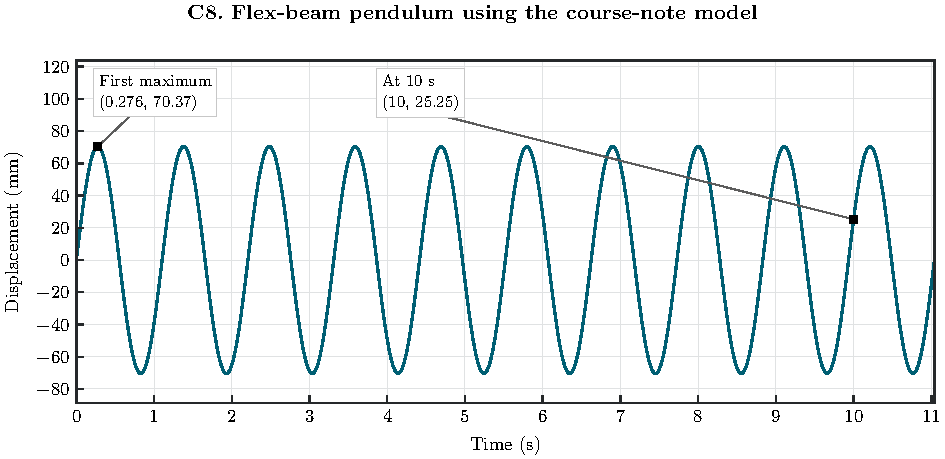
\includegraphics[width=0.95\linewidth,height=0.30\textheight,keepaspectratio,alt={C.8. Ten-cycle flex-beam pendulum response with markers at the first maximum and at ten seconds.}]{figures/generated/solutions/C8.pdf}
\caption{C.8. Ten-cycle response with data markers at the first maximum and at \(t=10\ \mathrm{s}\).}
\end{figure}

\[
\boxed{N_{\mathrm{osc}}=10,\quad t_{\mathrm{end}}=12.18\ \mathrm{s},\quad
u_{\max}=77.6\ \mathrm{mm}\ \text{at}\ t=0.304\ \mathrm{s}}
\qquad\text{(C.8.8.a)}
\]

\[
\boxed{u(10\ \mathrm{s})=75.5\ \mathrm{mm}}
\qquad\text{(C.8.8.b)}
\]

\matlabcaption{C.8 response plot.}
\begin{matlabcode}
L=.568; M=42; mp=.018; vp=935; E=200e9; h=.003; b=.037; g=9.81;
Nosc=10; t1=10;
I=b*h^3/12; k=3*E*I/L^3; Mt=M+mp;
v0=mp*vp/Mt; P=Mt*g; lam=sqrt(P/(E*I));
kT=P/(L-tanh(lam*L)/lam); wn=sqrt(kT/Mt); tau=2*pi/wn;
t=linspace(0,Nosc*tau,2000); A=1000*v0/wn; u=A*sin(wn*t);
plot(t,u,'Color',[0 .427 .459],'LineWidth',1.5);
hold on; tmax=pi/(2*wn); plot(tmax,A,'ks');
plot(t1,A*sin(wn*t1),'ks'); grid on;
xlabel('Time (s)'); ylabel('Displacement (mm)');
\end{matlabcode}

Problem A.3 models a simple pendulum, while C.8 includes the cantilever elastic stiffness in addition to the gravity contribution. The impact velocities are nearly identical. The C.8 frequency follows from the lateral stiffness of a beam under tensile preload, whereas A.3 uses the rigid-link pendulum relation.

\begin{center}
\small
\begin{tabular}{@{}lrrr@{}}
\toprule
Quantity & C.8 & A.3 & Unit \\
\midrule
\(\dot u_0\) & \(0.401\) & \(0.400\) & \(\mathrm{m/s}\) \\
\(\omega_n\) & \(5.16\) & \(4.17\) & \(\mathrm{rad/s}\) \\
\(\tau\) & \(1.218\) & \(1.508\) & \(\mathrm{s}\) \\
\(\lvert u\rvert_{\max}\) & \(77.6\) & \(95.9\) & \(\mathrm{mm}\) \\
\(u(10\ \mathrm{s})\) & \(75.5\) & \(-70.6\) & \(\mathrm{mm}\) \\
\bottomrule
\end{tabular}
\end{center}

The post-impact speeds differ by less than one percent. The flex-beam pendulum has a \(23.8\%\) higher natural frequency and a \(19.1\%\) smaller response amplitude than A.3. Its ten-second response is positive, whereas the A.3 response is negative because the two systems have different frequencies, periods, lengths, and impact data. The comparison shows the effect of the flex-beam model, but it does not isolate flexural stiffness because the lengths and impact parameters also differ. The C.8 amplitude is approximately \(0.137L\); the small-deflection, massless-beam assumptions still limit the physical accuracy of this linear response.

\[
\boxed{\omega_{n,\mathrm{FBP}}>\omega_{n,\mathrm{A.3}},\qquad
\lvert u\rvert_{\max,\mathrm{FBP}}<\lvert u\rvert_{\max,\mathrm{A.3}}}
\qquad\text{(C.8.9)}
\]
